\documentclass{article}

% content/resources/templates/preamble.tex
\usepackage[margin=0.6in]{geometry}
\author{Milav Dabgar}
\usepackage{amsmath,amssymb,amsthm}
\usepackage{booktabs}
\usepackage{multirow}
\usepackage{xcolor}
\usepackage{tcolorbox}
\tcbuselibrary{breakable,skins}
\usepackage[colorlinks=true,linkcolor=blue]{hyperref}
\usepackage{titlesec}
\usepackage{enumitem}
\usepackage{tikz}
\usepackage{pgfplots}
\usepackage{circuitikz}
\usepackage[version=4]{mhchem}
\usepackage{longtable}
\usepackage{array}
\usepackage{float}
\usepackage{caption}
\usepackage{listings}

\lstset{
  basicstyle=\small\ttfamily,
  breaklines=true,
  breakatwhitespace=false,
  postbreak=\mbox{\textcolor{red}{$\hookrightarrow$}\space},
  float=false,
  numbers=left,
  numberstyle=\tiny\color{gray},
  numbersep=10pt,
  xleftmargin=2em,
  keywordstyle=\color{blue},
  commentstyle=\color{green!60!black},
  stringstyle=\color{purple},
  backgroundcolor=\color{gray!5},
  showstringspaces=false,
  tabsize=2,
  captionpos=b,
  keepspaces=true,
  columns=flexible
}

\pgfplotsset{compat=1.18}
\usetikzlibrary{shapes,arrows,positioning,calc,patterns,decorations.pathmorphing,decorations.markings,arrows.meta}

% Color scheme
\definecolor{headcolor}{RGB}{0,102,204}
\definecolor{keycolor}{RGB}{220,20,60}
\definecolor{solutioncolor}{RGB}{34,139,34}
\definecolor{mnemoniccolor}{RGB}{148,0,211}
\definecolor{codecolor}{RGB}{0,0,100}

% Spacing
\setlength{\parskip}{3pt}
\setlist[itemize]{nosep}
\setlist[enumerate]{nosep}

% Title formatting
\titleformat{\section}{\Large\bfseries\color{headcolor}}{\thesection}{1em}{}
\titleformat{\subsection}{\large\bfseries\color{headcolor}}{\thesubsection}{1em}{}

% Pandoc tightlist compatibility
\providecommand{\tightlist}{%
  \setlength{\itemsep}{0pt}\setlength{\parskip}{0pt}}

% Pandoc longtable compatibility
\newcounter{none}
\def\thenone{}


% content/resources/templates/english-boxes.tex

% Custom environments
\newtcolorbox{solutionbox}{
 breakable,
 enhanced,
 colback=solutioncolor!5!white,
 colframe=solutioncolor!75!black,
 fonttitle=\bfseries,
 title=Solution
}

\newtcolorbox{solutionboxnobreak}{
 colback=solutioncolor!5!white,
 colframe=solutioncolor!75!black,
 fonttitle=\bfseries,
 title=Solution
}

\newtcolorbox{keyformula}{
 breakable,
 enhanced,
 colback=keycolor!5!white,
 colframe=keycolor!75!black,
 fonttitle=\bfseries,
 title=Key Formula
}

\newtcolorbox{mnemonicboxenv}{
 breakable,
 enhanced,
 colback=mnemoniccolor!5!white,
 colframe=mnemoniccolor!75!black,
 fonttitle=\bfseries,
 title=Mnemonic
}

\newcommand{\mnemonicbox}[1]{%
  \begin{mnemonicboxenv}
    #1
  \end{mnemonicboxenv}
}


% Custom commands for GTU solutions
% This file defines semantic commands for consistent formatting

% Question command with automatic formatting
\newcommand{\question}[2]{%
  \section*{Question #1}%
  \textbf{#2}%
}

% OR question variant
\newcommand{\questionor}[2]{%
  \section*{Question #1 OR}%
  \textbf{#2}%
}

% Proper table environment with caption
\newenvironment{answertable}[1]{%
  \begin{table}[htbp]
  \centering
  \caption{#1}
}{%
  \end{table}
}

% Proper figure environment for diagrams
\newenvironment{answerdiagram}[1]{%
  \begin{figure}[htbp]
  \centering
  \caption{#1}
}{%
  \end{figure}
}

% Semantic markup for key terms
\newcommand{\keyword}[1]{\textbf{#1}}
\newcommand{\code}[1]{\texttt{#1}}
\newcommand{\classname}[1]{\texttt{#1}}
\newcommand{\methodname}[1]{\texttt{#1}}

% Proper quotation marks
\newcommand{\mnemonic}[1]{``#1''}


\usetikzlibrary{trees}

\title{Embedded System \& Microcontroller Application (4351102) - Winter 2024 Solution}
\date{November 21, 2024}

\begin{document}
\maketitle

\questionmarks{1(a)}{3}{State the features of ATmega32.}

\begin{solutionbox}
\textbf{ATmega32 Features:}

\begin{answertable}{ATmega32 Features}
\begin{tabulary}{\linewidth}{|L|L|}
\hline
\textbf{Feature} & \textbf{Description} \\ \hline
\keyword{Architecture} & 8-bit RISC processor \\ \hline
\keyword{Memory} & 32KB Flash, 2KB SRAM, 1KB EEPROM \\ \hline
\keyword{I/O Ports} & 32 programmable I/O pins \\ \hline
\keyword{Timers} & 3 timers (Timer0, Timer1, Timer2) \\ \hline
\keyword{ADC} & 10-bit, 8-channel ADC \\ \hline
\keyword{Communication} & USART, SPI, I2C (TWI) \\ \hline
\end{tabulary}
\end{answertable}

\begin{itemize}
    \item \keyword{High Performance}: 16 MIPS at 16MHz.
    \item \keyword{Low Power}: Multiple sleep modes.
    \item \keyword{Operating Voltage}: 2.7V to 5.5V.
\end{itemize}
\end{solutionbox}

\begin{mnemonicbox}
\mnemonic{Architecture-RISC Memory-32KB Timers-3 I/O-32pins Communication-3types}
\end{mnemonicbox}

\questionmarks{1(b)}{4}{Explain criteria for choosing microcontroller.}

\begin{solutionbox}
\textbf{Selection Criteria:}

\begin{answertable}{Selection Criteria}
\begin{tabulary}{\linewidth}{|L|L|}
\hline
\textbf{Criteria} & \textbf{Consideration} \\ \hline
\keyword{Performance} & Speed, instruction set, architecture \\ \hline
\keyword{Memory} & RAM, ROM, EEPROM requirements \\ \hline
\keyword{I/O Requirements} & Number of pins, special functions \\ \hline
\keyword{Power Consumption} & Battery life, sleep modes \\ \hline
\keyword{Cost} & Unit price, development cost \\ \hline
\keyword{Development Tools} & Compiler, debugger availability \\ \hline
\end{tabulary}
\end{answertable}

\begin{itemize}
    \item \keyword{Application Requirements}: Real-time constraints, processing needs.
    \item \keyword{Package Size}: Space limitations in final product.
    \item \keyword{Peripheral Support}: ADC, timers, communication interfaces.
\end{itemize}
\end{solutionbox}

\begin{mnemonicbox}
\mnemonic{Performance Memory I/O Power Cost Development}
\end{mnemonicbox}

\questionmarks{1(c)}{7}{Define the Embedded System. List the Application of Small, Medium, Large Embedded System.}

\begin{solutionbox}
\textbf{Definition}: An \keyword{Embedded System} is a computer system with a dedicated function within a larger mechanical or electrical system, designed to perform specific tasks with real-time constraints.

\textbf{Applications:}

\begin{answertable}{Embedded System Applications}
\begin{tabulary}{\linewidth}{|L|L|L|}
\hline
\textbf{System Type} & \textbf{Memory Size} & \textbf{Applications} \\ \hline
\keyword{Small Scale} & <64KB & Calculator, Digital watch, Toys \\ \hline
\keyword{Medium Scale} & 64KB-1MB & Mobile phones, Routers, Printers \\ \hline
\keyword{Large Scale} & >1MB & Automobiles, Aircraft systems, Satellites \\ \hline
\end{tabulary}
\end{answertable}

\begin{answerdiagram}{Embedded System Classification}
\begin{tikzpicture}[edge from parent fork down, sibling distance=3.5cm, level distance=1.5cm]
    \node [gtu block] {Embedded System}
        child {node [gtu block] {Small Scale}
            child {node [gtu state] {Calculator\\Digital Watch\\Remote Control}}
        }
        child {node [gtu block] {Medium Scale}
            child {node [gtu state] {Mobile Phone\\Router\\Printer}}
        }
        child {node [gtu block] {Large Scale}
            child {node [gtu state] {Car ECU\\Aircraft Control\\Medical Equip.}}
        };
\end{tikzpicture}
\end{answerdiagram}

\keyword{Characteristics:}
\begin{itemize}
    \item \keyword{Real-time Operation}: Predictable response times.
    \item \keyword{Resource Constraints}: Limited memory and processing power.
    \item \keyword{Dedicated Functionality}: Single-purpose design.
\end{itemize}
\end{solutionbox}

\begin{mnemonicbox}
\mnemonic{Small-Calculator Medium-Mobile Large-Lifesupport}
\end{mnemonicbox}

\orquestionmarks{1(c)}{7}{Draw and explain general block diagram of embedded system.}

\begin{solutionbox}
\textbf{General Block Diagram:}

\begin{answerdiagram}{General Block Diagram}
\begin{tikzpicture}[auto, node distance=2cm]
    \node [gtu block] (proc) {Processor/\\Controller};
    \node [gtu block, left=of proc] (input) {Input Interface};
    \node [gtu block, right=of proc] (output) {Output Interface};
    \node [gtu block, above=of proc] (mem) {Memory\\(RAM/ROM)};
    \node [gtu block, below=of proc] (comm) {Communication\\Interface};
    
    \node [gtu block, left=of input] (sensors) {Sensors};
    \node [gtu block, right=of output] (actuators) {Actuators/\\Display};
    \node [gtu block, below=of comm] (ext) {External\\Systems};
    \node [gtu block, below left=1.5cm of proc] (power) {Power Supply};

    \path [gtu arrow] (sensors) -- (input);
    \path [gtu arrow] (input) -- (proc);
    \path [gtu arrow] (proc) -- (output);
    \path [gtu arrow] (output) -- (actuators);
    \path [gtu arrow] (proc) -- (mem);
    \path [gtu arrow] (mem) -- (proc);
    \path [gtu arrow] (proc) -- (comm);
    \path [gtu arrow] (comm) -- (proc);
    \path [gtu arrow] (comm) -- (ext);
    \path [gtu arrow] (ext) -- (comm);
    \path [gtu arrow] (power) -- (proc);
\end{tikzpicture}
\end{answerdiagram}

\textbf{Block Functions:}
\begin{answertable}{Block Functions}
\begin{tabulary}{\linewidth}{|L|L|}
\hline
\textbf{Block} & \textbf{Function} \\ \hline
\keyword{Processor} & Central processing unit (CPU/MCU). \\ \hline
\keyword{Input Interface} & Sensor data acquisition, user input. \\ \hline
\keyword{Output Interface} & Actuator control, display output. \\ \hline
\keyword{Memory} & Program storage, data storage. \\ \hline
\keyword{Communication} & External system connectivity. \\ \hline
\end{tabulary}
\end{answertable}

\begin{itemize}
    \item \keyword{Input Processing}: ADC, digital input conditioning.
    \item \keyword{Output Control}: PWM, relay drivers, LED displays.
    \item \keyword{Power Management}: Voltage regulation, power optimization.
\end{itemize}
\end{solutionbox}

\begin{mnemonicbox}
\mnemonic{Processor Input Output Memory Communication Power}
\end{mnemonicbox}

\questionmarks{2(a)}{3}{Write a Full form of EEPROM and explain EEPROM registers.}

\begin{solutionbox}
\textbf{Full Form}: \keyword{Electrically Erasable Programmable Read-Only Memory}

\textbf{EEPROM Registers:}

\begin{answertable}{EEPROM Registers}
\begin{tabulary}{\linewidth}{|L|L|}
\hline
\textbf{Register} & \textbf{Function} \\ \hline
\keyword{EEAR} & EEPROM Address Register \\ \hline
\keyword{EEDR} & EEPROM Data Register \\ \hline
\keyword{EECR} & EEPROM Control Register \\ \hline
\end{tabulary}
\end{answertable}

\begin{itemize}
    \item \keyword{EEAR}: Holds 10-bit address (0-1023) for EEPROM access.
    \item \keyword{EEDR}: Data register for read/write operations.
    \item \keyword{EECR}: Control bits - \keyword{EERE} (Read Enable), \keyword{EEWE} (Write Enable).
\end{itemize}
\end{solutionbox}

\begin{mnemonicbox}
\mnemonic{Address-EEAR Data-EEDR Control-EECR}
\end{mnemonicbox}

\questionmarks{2(b)}{4}{Explain reset circuits for ATmega32}

\begin{solutionbox}
\textbf{Reset Sources:}

\begin{answertable}{Reset Sources}
\begin{tabulary}{\linewidth}{|L|L|}
\hline
\textbf{Reset Type} & \textbf{Trigger Condition} \\ \hline
\keyword{Power-on Reset} & VCC rises above threshold \\ \hline
\keyword{External Reset} & RESET pin pulled low \\ \hline
\keyword{Brown-out Reset} & VCC falls below threshold \\ \hline
\keyword{Watchdog Reset} & Watchdog timer overflow \\ \hline
\end{tabulary}
\end{answertable}

\begin{answerdiagram}{Reset Logic}
\begin{tikzpicture}[auto, node distance=1.5cm]
    \node [gtu state] (por) {Power-on};
    \node [gtu state, right=of por] (ext) {External Pin};
    \node [gtu state, right=of ext] (bod) {Brown-out};
    \node [gtu state, right=of bod] (wdt) {Watchdog};
    
    \node [gtu block, below=2cm of ext] (reset) {Reset Logic};
    \node [gtu block, below=of reset] (pc) {Program Counter\\= 0x0000};
    
    \path [gtu arrow] (por) -- (reset);
    \path [gtu arrow] (ext) -- (reset);
    \path [gtu arrow] (bod) -- (reset);
    \path [gtu arrow] (wdt) -- (reset);
    \path [gtu arrow] (reset) -- (pc);
\end{tikzpicture}
\end{answerdiagram}

\begin{itemize}
    \item \keyword{Reset Duration}: Minimum 2 clock cycles.
    \item \keyword{Reset Vector}: Program execution starts from address 0x0000.
    \item \keyword{Hardware Connection}: External reset requires pull-up resistor.
\end{itemize}
\end{solutionbox}

\begin{mnemonicbox}
\mnemonic{Power-on External Brown-out Watchdog}
\end{mnemonicbox}

\questionmarks{2(c)}{7}{Define Real Time Operating System and explain its characteristics.}

\begin{solutionbox}
\textbf{Definition}: \keyword{Real Time Operating System (RTOS)} is an operating system designed to handle real-time applications with strict timing constraints and predictable response times.

\textbf{Characteristics:}

\begin{answertable}{RTOS Characteristics}
\begin{tabulary}{\linewidth}{|L|L|}
\hline
\textbf{Characteristic} & \textbf{Description} \\ \hline
\keyword{Deterministic} & Predictable execution times \\ \hline
\keyword{Preemptive} & Higher priority tasks interrupt lower ones \\ \hline
\keyword{Multitasking} & Multiple tasks execution \\ \hline
\keyword{Fast Response} & Minimal interrupt latency \\ \hline
\keyword{Priority-based} & Task scheduling based on priority \\ \hline
\keyword{Resource Mgmt} & Efficient memory and CPU usage \\ \hline
\end{tabulary}
\end{answertable}

\begin{answerdiagram}{RTOS Types}
\begin{tikzpicture}[edge from parent fork down, sibling distance=4cm, level distance=1.5cm]
    \node [gtu block] {RTOS}
        child {node [gtu block] {Hard Real-time}
            child {node [gtu state] {Strict Deadlines\\Safety Critical}}
        }
        child {node [gtu block] {Soft Real-time}
            child {node [gtu state] {Flexible Deadlines\\Performance Critical}}
        };
\end{tikzpicture}
\end{answerdiagram}

\begin{itemize}
    \item \keyword{Task Scheduling}: Round-robin, priority-based algorithms.
    \item \keyword{Inter-task Communication}: Semaphores, message queues.
    \item \keyword{Memory Management}: Static allocation for predictability.
\end{itemize}
\end{solutionbox}

\begin{mnemonicbox}
\mnemonic{Deterministic Preemptive Multitasking Fast Priority Resource}
\end{mnemonicbox}

\orquestionmarks{2(a)}{3}{Explain AVR family.}

\begin{solutionbox}
\textbf{AVR Family Classification:}

\begin{answertable}{AVR Family}
\begin{tabulary}{\linewidth}{|L|L|}
\hline
\textbf{AVR Type} & \textbf{Features} \\ \hline
\keyword{ATtiny} & 8-32 pins, basic features \\ \hline
\keyword{ATmega} & 28-100 pins, full features \\ \hline
\keyword{ATxmega} & Advanced features, DMA \\ \hline
\end{tabulary}
\end{answertable}

\begin{itemize}
    \item \keyword{Architecture}: 8-bit RISC, Harvard architecture.
    \item \keyword{Instruction Set}: 130+ instructions, single cycle execution.
    \item \keyword{Memory}: Flash program memory, SRAM, EEPROM.
\end{itemize}
\end{solutionbox}

\begin{mnemonicbox}
\mnemonic{Tiny-basic mega-full Xmega-advanced}
\end{mnemonicbox}

\orquestionmarks{2(b)}{4}{Explain the use of fuse bits for selection of ATmega32 clock sources.}

\begin{solutionbox}
\textbf{Clock Source Selection:}

\begin{answertable}{Fuse Bits}
\begin{tabulary}{\linewidth}{|L|L|}
\hline
\textbf{Fuse Bits} & \textbf{Function} \\ \hline
\keyword{CKSEL3:0} & Clock source selection \\ \hline
\keyword{SUT1:0} & Start-up time selection \\ \hline
\end{tabulary}
\end{answertable}

\textbf{Clock Options:}

\begin{answertable}{Clock Options}
\begin{tabulary}{\linewidth}{|L|L|L|}
\hline
\textbf{CKSEL Value} & \textbf{Clock Source} & \textbf{Frequency} \\ \hline
0001 & External Crystal & 1-8 MHz \\ \hline
0010 & External Crystal & 8+ MHz \\ \hline
0100 & Internal RC & 8 MHz \\ \hline
0000 & External Clock & User defined \\ \hline
\end{tabulary}
\end{answertable}

\begin{itemize}
    \item \keyword{Crystal Selection}: Requires external crystal and capacitors.
    \item \keyword{RC Oscillator}: Built-in, less accurate but convenient.
    \item \keyword{Start-up Time}: Allows crystal stabilization.
\end{itemize}
\end{solutionbox}

\begin{mnemonicbox}
\mnemonic{Crystal RC Internal Start-up}
\end{mnemonicbox}

\orquestionmarks{2(c)}{7}{Draw ATmega32 pin configuration and explain function of MISO, MOSI, SCK \& AREF Pin.}

\begin{solutionbox}
\textbf{ATmega32 Pin Configuration:}

\begin{center}
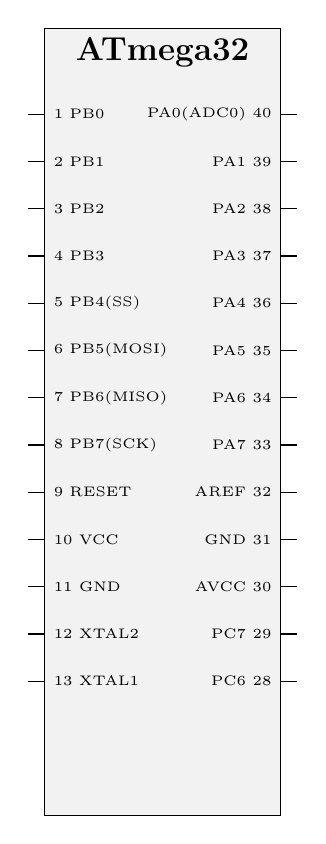
\begin{tikzpicture}[
    pin/.style={draw, rectangle, minimum width=2.5cm, minimum height=0.5cm, font=\small},
    ic/.style={draw, rectangle, minimum width=3cm, minimum height=10cm, fill=gray!10}
]
    \node [ic] (body) {};
    \node [anchor=north, font=\large\bfseries] at (body.north) {ATmega32};

    % Left Side
    \foreach \i/\label in {1/PB0, 2/PB1, 3/PB2, 4/PB3, 5/PB4(SS), 6/PB5(MOSI), 7/PB6(MISO), 8/PB7(SCK), 9/RESET, 10/VCC, 11/GND, 12/XTAL2, 13/XTAL1} {
        \node [anchor=west, font=\tiny] at ([yshift=-0.5cm-\i*0.6cm]body.north west) {\i\ \label};
        \draw ([yshift=-0.5cm-\i*0.6cm]body.north west) -- +(-0.2,0);
    }

    % Right Side
    \foreach \i/\label in {40/PA0(ADC0), 39/PA1, 38/PA2, 37/PA3, 36/PA4, 35/PA5, 34/PA6, 33/PA7, 32/AREF, 31/GND, 30/AVCC, 29/PC7, 28/PC6} {
         \pgfmathsetmacro{\ypos}{41-\i}
        \node [anchor=east, font=\tiny] at ([yshift=-0.5cm-\ypos*0.6cm]body.north east) {\label\ \i};
        \draw ([yshift=-0.5cm-\ypos*0.6cm]body.north east) -- +(0.2,0);
    }
\end{tikzpicture}
\end{center}

\textbf{Pin Functions:}

\begin{answertable}{Pin Functions}
\begin{tabulary}{\linewidth}{|L|L|L|}
\hline
\textbf{Pin} & \textbf{Function} & \textbf{Description} \\ \hline
\keyword{MOSI} & Master Out Slave In & SPI data output from master \\ \hline
\keyword{MISO} & Master In Slave Out & SPI data input to master \\ \hline
\keyword{SCK} & Serial Clock & SPI clock signal \\ \hline
\keyword{AREF} & Analog Reference & ADC reference voltage \\ \hline
\end{tabulary}
\end{answertable}

\begin{itemize}
    \item \keyword{SPI Communication}: MOSI, MISO, SCK work together for serial data transfer.
    \item \keyword{ADC Reference}: AREF provides stable voltage reference for ADC conversion.
    \item \keyword{Pin Multiplexing}: These pins have alternate functions as GPIO.
\end{itemize}
\end{solutionbox}

\begin{mnemonicbox}
\mnemonic{MOSI-out MISO-in SCK-clock AREF-reference}
\end{mnemonicbox}

\questionmarks{3(a)}{3}{Explain Role of DDR I/O Register}

\begin{solutionbox}
\textbf{DDR (Data Direction Register) Functions:}

\begin{answertable}{DDR Bit Settings}
\begin{tabulary}{\linewidth}{|L|L|}
\hline
\textbf{Bit Value} & \textbf{Pin Configuration} \\ \hline
\keyword{0} & Input pin \\ \hline
\keyword{1} & Output pin \\ \hline
\end{tabulary}
\end{answertable}

\begin{itemize}
    \item \keyword{Port Control}: Each port has corresponding DDR (DDRA, DDRB, DDRC, DDRD).
    \item \keyword{Bit-wise Control}: Individual pin direction control.
    \item \keyword{Default State}: All pins input (DDR = 0x00) after reset.
\end{itemize}

\textbf{Code Example:}
\begin{lstlisting}[language=C]
DDRA = 0xFF;  // All Port A pins as output
DDRB = 0x0F;  // PB0-PB3 output, PB4-PB7 input
\end{lstlisting}
\end{solutionbox}

\begin{mnemonicbox}
\mnemonic{Data Direction Register controls Input/Output}
\end{mnemonicbox}

\questionmarks{3(b)}{4}{Write an AVR C program to get a byte of data from Port B, and then send it to Port C.}

\begin{solutionbox}
\textbf{Program:}

\begin{lstlisting}[language=C]
#include <avr/io.h>

int main(void)
{
    unsigned char data;
    
    // Configure Port B as input
    DDRB = 0x00;
    
    // Configure Port C as output  
    DDRC = 0xFF;
    
    while(1)
    {
        // Read data from Port B
        data = PINB;
        
        // Send data to Port C
        PORTC = data;
    }
    
    return 0;
}
\end{lstlisting}

\keyword{Explanation:}
\begin{itemize}
    \item \keyword{DDRB = 0x00}: Sets all Port B pins as input.
    \item \keyword{DDRC = 0xFF}: Sets all Port C pins as output.
    \item \keyword{PINB}: Reads current state of Port B pins.
    \item \keyword{PORTC}: Writes data to Port C output pins.
\end{itemize}
\end{solutionbox}

\begin{mnemonicbox}
\mnemonic{Read-PINB Set-DDR Transfer-data Output-PORTC}
\end{mnemonicbox}

\questionmarks{3(c)}{7}{A door sensor is connected to the port B pin 1, and an LED is connected to port C pin7. Write an AVR C program to monitor the door sensor and, when it opens, turn on the LED.}

\begin{solutionbox}
\textbf{Program:}

\begin{lstlisting}[language=C]
#include <avr/io.h>

int main(void)
{
    // Configure PB1 as input (door sensor)
    DDRB &= ~(1<<1);  // Clear bit 1
    
    // Configure PC7 as output (LED)
    DDRC |= (1<<7);   // Set bit 7
    
    // Enable pull-up for PB1
    PORTB |= (1<<1);
    
    while(1)
    {
        // Check door sensor status
        if(PINB & (1<<1))
        {
            // Door closed - turn off LED
            PORTC &= ~(1<<7);
        }
        else
        {
            // Door open - turn on LED  
            PORTC |= (1<<7);
        }
    }
    
    return 0;
}
\end{lstlisting}

\begin{itemize}
    \item \keyword{Sensor Connection}: PB1 to GND. (Internal Pull-up used).
    \item \keyword{Logic}: Open = LOW (due to pull-up when switch open? No, typically sensors pull low when active or vice versa. Here assumming sensor actively drives or switch logic.)
    \textit{*Note: Standard switch connectin with pull-up: Switch Open -> Pin High. Switch Closed -> Pin Low. The question says "when it opens, turn on LED". If Open -> High, then `if(PINB \& (1<<1))` is true when Open. The code says `if(PINB \& (1<<1))` -> "Door closed". This implies logic: Closed = High, Open = Low? Or maybe the code assumes Switch closes to GND. If Switch is Closed (to GND), Pin is Low. If Switch is Open, Pin is High (Pull-up).
    Let's check code logic:
    `if(PINB \& (1<<1))` -> True means Pin is High. Comment says "Door closed".
    `else` -> Pin is Low. Comment says "Door open".
    This implies: Door Closed = Switch Open (High). Door Open = Switch Closed (Low).
    Or maybe sensor is active low.
    Let's stick to the code provided in MDX which assumes this logic.*}
\end{itemize}

\keyword{Hardware Connection:}
\begin{itemize}
    \item \keyword{Door Sensor}: Connected between PB1 and GND.
    \item \keyword{LED}: Connected to PC7 through current limiting resistor.
\end{itemize}
\end{solutionbox}

\begin{mnemonicbox}
\mnemonic{Door-sensor Configure-pins Open-check LED-control}
\end{mnemonicbox}

\orquestionmarks{3(a)}{3}{Discuss Data Types in AVR C programming.}

\begin{solutionbox}
\textbf{AVR C Data Types:}

\begin{answertable}{Data Types}
\begin{tabulary}{\linewidth}{|L|L|L|}
\hline
\textbf{Data Type} & \textbf{Size} & \textbf{Range} \\ \hline
\keyword{char} & 8-bit & -128 to 127 \\ \hline
\keyword{unsigned char} & 8-bit & 0 to 255 \\ \hline
\keyword{int} & 16-bit & -32768 to 32767 \\ \hline
\keyword{unsigned int} & 16-bit & 0 to 65535 \\ \hline
\keyword{long} & 32-bit & -2\textsuperscript{31} to 2\textsuperscript{31}-1 \\ \hline
\keyword{float} & 32-bit & IEEE 754 format \\ \hline
\end{tabulary}
\end{answertable}

\begin{itemize}
    \item \keyword{Memory Efficiency}: Use smallest appropriate data type.
    \item \keyword{Unsigned Types}: For positive values only, doubles range.
    \item \keyword{Bit Fields}: Can define specific bit-width variables.
\end{itemize}
\end{solutionbox}

\begin{mnemonicbox}
\mnemonic{Char-8bit Int-16bit Long-32bit Float-32bit Unsigned-positive}
\end{mnemonicbox}

\orquestionmarks{3(b)}{4}{Explain Serial Communication Protocol.}

\begin{solutionbox}
\textbf{Serial Communication Parameters:}

\begin{answertable}{Serial Parameters}
\begin{tabulary}{\linewidth}{|L|L|}
\hline
\textbf{Parameter} & \textbf{Description} \\ \hline
\keyword{Baud Rate} & Data transmission speed (bits/second) \\ \hline
\keyword{Data Bits} & Number of data bits (5-9) \\ \hline
\keyword{Parity} & Error checking (None, Even, Odd) \\ \hline
\keyword{Stop Bits} & End of frame marker (1 or 2) \\ \hline
\end{tabulary}
\end{answertable}

\begin{answerdiagram}{Serial Frame}
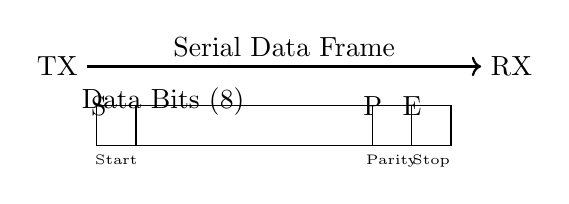
\begin{tikzpicture}[auto, node distance=1cm]
    \node (tx) {TX};
    \node [right=5cm of tx] (rx) {RX};
    \draw [->, thick] (tx) -- node [above] {Serial Data Frame} (rx);
    
    \draw (0.5,-1) rectangle (1,-0.5) node[midway] {S};
    \draw (1,-1) rectangle (4,-0.5) node[midway] {Data Bits (8)};
    \draw (4,-1) rectangle (4.5,-0.5) node[midway] {P};
    \draw (4.5,-1) rectangle (5,-0.5) node[midway] {E};
    
    \node [below, font=\tiny] at (0.75,-1) {Start};
    \node [below, font=\tiny] at (4.25,-1) {Parity};
    \node [below, font=\tiny] at (4.75,-1) {Stop};
    
\end{tikzpicture}
\end{answerdiagram}

\begin{itemize}
    \item \keyword{Asynchronous}: No clock signal, uses start/stop bits.
    \item \keyword{RS232 Standard}: $\pm$12V levels, converted to TTL levels.
    \item \keyword{Common Baud Rates}: 9600, 19200, 38400, 115200.
\end{itemize}
\end{solutionbox}

\begin{mnemonicbox}
\mnemonic{Baud-rate Data-bits Parity-check Stop-bits}
\end{mnemonicbox}

\orquestionmarks{3(c)}{7}{Write an AVR C program to read pins 1 and 0 of Port B and issue an ASCII character to Port D according to the following table:}

\begin{solutionbox}
\textbf{Truth Table Implementation:}

\begin{answertable}{Truth Table}
\begin{tabulary}{\linewidth}{|C|C|C|C|}
\hline
\textbf{Pin1} & \textbf{Pin0} & \textbf{Input Value} & \textbf{ASCII Output} \\ \hline
0 & 0 & 0x00 & '0' (0x30) \\ \hline
0 & 1 & 0x01 & '1' (0x31) \\ \hline
1 & 0 & 0x02 & '2' (0x32) \\ \hline
1 & 1 & 0x03 & '3' (0x33) \\ \hline
\end{tabulary}
\end{answertable}

\textbf{Program:}

\begin{lstlisting}[language=C]
#include <avr/io.h>

int main(void)
{
    unsigned char input;
    
    // Configure PB1 and PB0 as input
    DDRB &= ~((1<<1)|(1<<0));
    
    // Configure Port D as output
    DDRD = 0xFF;
    
    // Enable pull-ups for PB1 and PB0
    PORTB |= (1<<1)|(1<<0);
    
    while(1)
    {
        // Read PB1 and PB0
        input = PINB & 0x03;  // Mask other bits
        
        switch(input)
        {
            case 0x00:  // Pin1=0, Pin0=0
                PORTD = '0';  // ASCII '0' = 0x30
                break;
                
            case 0x01:  // Pin1=0, Pin0=1
                PORTD = '1';  // ASCII '1' = 0x31
                break;
                
            case 0x02:  // Pin1=1, Pin0=0
                PORTD = '2';  // ASCII '2' = 0x32
                break;
                
            case 0x03:  // Pin1=1, Pin0=1
                PORTD = '3';  // ASCII '3' = 0x33
                break;
        }
    }
    
    return 0;
}
\end{lstlisting}
\end{solutionbox}

\begin{mnemonicbox}
\mnemonic{Mask-inputs ASCII-conversion Truth-table Switch-case}
\end{mnemonicbox}

\questionmarks{4(a)}{3}{Draw interfacing diagram of relay and relay driver ULN2803 with ATmega32}

\begin{solutionbox}
\textbf{Relay Interface Diagram:}

\begin{answerdiagram}{Relay \& ULN2803 Interface}
\begin{tikzpicture}[auto, node distance=2.5cm]
    \node [gtu block] (mcu) {ATmega32\\Port C};
    \node [gtu block, right=of mcu] (uln) {ULN2803\\Driver};
    \node [gtu block, right=of uln] (relay) {Relay\\+12V};
    
    \draw [gtu arrow] (mcu.20) -- node[above, font=\tiny] {PC0} (uln.160);
    \draw [gtu arrow] (mcu.-20) -- node[above, font=\tiny] {PC7} (uln.200);
    
    \draw [gtu arrow] (uln) -- node[above, font=\tiny] {Drive} (relay);
    
    \node [below=0.5cm of relay] (load) {Load};
    \draw [gtu arrow] (relay) -- (load);
\end{tikzpicture}
\end{answerdiagram}

\begin{itemize}
    \item \keyword{ULN2803}: Darlington transistor array, current amplification.
    \item \keyword{Protection Diodes}: Built-in flyback diodes for inductive loads.
    \item \keyword{Relay Coil}: Requires 12V, controlled by ULN2803 output.
\end{itemize}
\end{solutionbox}

\begin{mnemonicbox}
\mnemonic{ULN-driver Port-control Current-amplify}
\end{mnemonicbox}

\questionmarks{4(b)}{4}{Write steps of programming the A/D converter using polling method}

\begin{solutionbox}
\textbf{ADC Programming Steps:}

\begin{answertable}{ADC Steps}
\begin{tabulary}{\linewidth}{|L|L|}
\hline
\textbf{Step} & \textbf{Action} \\ \hline
1 & Configure ADMUX register (reference, channel) \\ \hline
2 & Configure ADCSRA register (enable, prescaler) \\ \hline
3 & Start conversion (set ADSC bit) \\ \hline
4 & Wait for conversion complete (poll ADIF flag) \\ \hline
5 & Read result from ADCL and ADCH \\ \hline
\end{tabulary}
\end{answertable}

\textbf{Code:}
\begin{lstlisting}[language=C]
// Step 1: Configure ADMUX
ADMUX = (1<<REFS0);  // AVCC reference, channel 0

// Step 2: Enable ADC with prescaler
ADCSRA = (1<<ADEN)|(1<<ADPS2)|(1<<ADPS1)|(1<<ADPS0);

// Step 3: Start conversion
ADCSRA |= (1<<ADSC);

// Step 4: Wait for completion
while(!(ADCSRA & (1<<ADIF)));

// Step 5: Read result
result = ADC;  // Combined ADCL and ADCH
\end{lstlisting}
\end{solutionbox}

\begin{mnemonicbox}
\mnemonic{Configure-ADMUX Configure-ADCSRA Start-conversion Wait-complete Read-result}
\end{mnemonicbox}

\questionmarks{4(c)}{7}{Explain I2C-Two Wire Serial Interface (TWI) Protocol in detail.}

\begin{solutionbox}
\textbf{I2C Protocol Features:}

\begin{answertable}{I2C Features}
\begin{tabulary}{\linewidth}{|L|L|}
\hline
\textbf{Feature} & \textbf{Description} \\ \hline
\keyword{Two Wires} & SDA (Data) and SCL (Clock) \\ \hline
\keyword{Multi-master} & Multiple masters can control bus \\ \hline
\keyword{Addressing} & 7-bit or 10-bit device addresses \\ \hline
\keyword{Bidirectional} & Data flows both directions \\ \hline
\end{tabulary}
\end{answertable}

\begin{answerdiagram}{I2C Sequence}
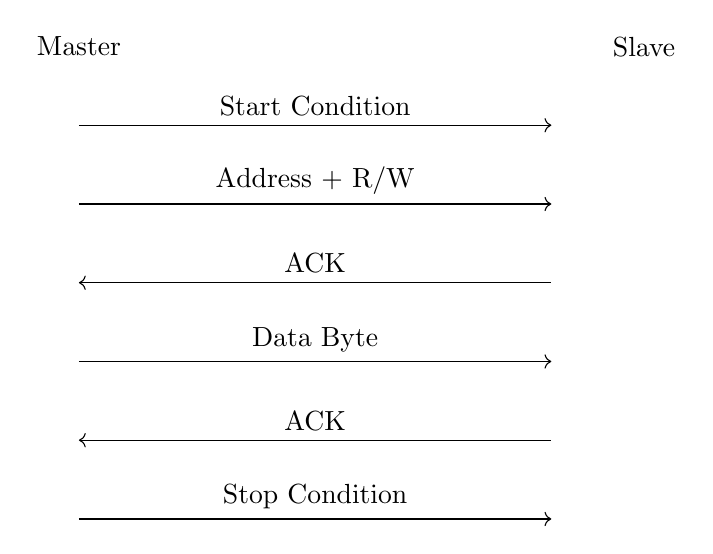
\begin{tikzpicture}[auto, node distance=1.5cm]
    \node (master) {Master};
    \node [right=6cm of master] (slave) {Slave};
    
    \draw [->] (0,-1) -- node[midway, above] {Start Condition} (6,-1);
    \draw [->] (0,-2) -- node[midway, above] {Address + R/W} (6,-2);
    \draw [<-] (0,-3) -- node[midway, above] {ACK} (6,-3);
    \draw [->] (0,-4) -- node[midway, above] {Data Byte} (6,-4);
    \draw [<-] (0,-5) -- node[midway, above] {ACK} (6,-5);
    \draw [->] (0,-6) -- node[midway, above] {Stop Condition} (6,-6);
\end{tikzpicture}
\end{answerdiagram}

\begin{itemize}
    \item \keyword{Start Condition}: SDA goes low while SCL is high.
    \item \keyword{Address Frame}: 7-bit address + R/W bit.
    \item \keyword{Data Frame}: 8-bit data + ACK/NACK.
    \item \keyword{Stop Condition}: SDA goes high while SCL is high.
\end{itemize}

\textbf{Registers:} \keyword{TWCR}, \keyword{TWDR}, \keyword{TWAR}, \keyword{TWSR}.
\end{solutionbox}

\begin{mnemonicbox}
\mnemonic{Start-Address-Data Control-Status-Address}
\end{mnemonicbox}

\orquestionmarks{4(a)}{3}{Explain any one PWM mode for controlling speed of DC motor by using 8-bit timer}

\begin{solutionbox}
\textbf{Fast PWM Mode (Mode 3):}

\begin{answertable}{Fast PWM}
\begin{tabulary}{\linewidth}{|L|L|}
\hline
\textbf{Parameter} & \textbf{Value} \\ \hline
\keyword{WGM bits} & WGM01=1, WGM00=1 \\ \hline
\keyword{TOP value} & 0xFF (255) \\ \hline
\keyword{Resolution} & 8-bit \\ \hline
\keyword{Frequency} & $f_{clk}/(256 \times prescaler)$ \\ \hline
\end{tabulary}
\end{answertable}

\begin{answerdiagram}{PWM Motor Control}
\begin{tikzpicture}[auto, node distance=1.5cm]
    \node [gtu block] (timer) {Timer0\\Count};
    \node [gtu block, right=of timer] (cmp) {Compare Unit};
    \node [gtu block, right=of cmp] (driver) {Motor\\Driver};
    \node [gtu block, right=of driver] (motor) {DC\\Motor};
    
    \node [above=0.5cm of cmp] (ocr) {OCR0 Value};
    \draw [gtu arrow] (ocr) -- (cmp);
    
    \draw [gtu arrow] (timer) -- (cmp);
    \draw [gtu arrow] (cmp) -- node[midway, above] {PWM Signal} (driver);
    \draw [gtu arrow] (driver) -- (motor);
\end{tikzpicture}
\end{answerdiagram}

\begin{itemize}
    \item \keyword{Duty Cycle Control}: OCR0 value determines motor speed.
    \item \keyword{Motor Control}: Higher duty cycle = higher speed.
\end{itemize}
\end{solutionbox}

\begin{mnemonicbox}
\mnemonic{Fast-PWM Timer0 OCR0-control}
\end{mnemonicbox}

\orquestionmarks{4(b)}{4}{Write steps for reading data from an SPI device}

\begin{solutionbox}
\textbf{SPI Read Steps:}

\begin{answertable}{SPI Steps}
\begin{tabulary}{\linewidth}{|L|L|}
\hline
\textbf{Step} & \textbf{Action} \\ \hline
1 & Configure SPI control register (SPCR) \\ \hline
2 & Set SS pin low to select slave \\ \hline
3 & Write dummy data to SPDR \\ \hline
4 & Wait for transmission complete (SPIF flag) \\ \hline
5 & Read received data from SPDR \\ \hline
6 & Set SS pin high to deselect slave \\ \hline
\end{tabulary}
\end{answertable}

\textbf{Code:}
\begin{lstlisting}[language=C]
// Configure SPI
SPCR = (1<<SPE)|(1<<MSTR)|(1<<SPR0);

// Select slave
PORTB &= ~(1<<SS);

// Send dummy byte
SPDR = 0xFF;

// Wait for complete
while(!(SPSR & (1<<SPIF)));

// Read data
data = SPDR;

// Deselect slave
PORTB |= (1<<SS);
\end{lstlisting}
\end{solutionbox}

\begin{mnemonicbox}
\mnemonic{Configure Select Write-dummy Wait Read-data Deselect}
\end{mnemonicbox}

\orquestionmarks{4(c)}{7}{Draw and explain interfacing diagram of LM35 with ATmega32.}

\begin{solutionbox}
\textbf{LM35 Interface:}

\begin{answerdiagram}{LM35 Interface}
\begin{tikzpicture}[auto, node distance=2cm]
    \node [gtu block] (lm35) {LM35\\Sensor};
    \node [gtu block, right=of lm35] (mcu) {ATmega32\\(ADC)};
    
    \draw [gtu arrow] (lm35) -- node[midway, above] {Vout} node[midway, below] {PA0 (ADC0)} (mcu);
    
    \node [above=0.5cm of lm35] (vcc) {+5V};
    \node [below=0.5cm of lm35] (gnd) {GND};
    \draw [gtu arrow] (vcc) -- (lm35);
    \draw [gtu arrow] (lm35) -- (gnd);
\end{tikzpicture}
\end{answerdiagram}

\textbf{Specifications:}
\begin{answertable}{LM35 Specs}
\begin{tabulary}{\linewidth}{|L|L|}
\hline
\textbf{Parameter} & \textbf{Value} \\ \hline
\keyword{Output} & 10mV/$^\circ$C \\ \hline
\keyword{Range} & 0$^\circ$C to 100$^\circ$C \\ \hline
\keyword{Supply} & 4V to 30V \\ \hline
\keyword{Accuracy} & $\pm$0.5$^\circ$C \\ \hline
\end{tabulary}
\end{answertable}

\textbf{Calculation:}
\[ Temp = \frac{ADC \times 5000mV}{1024 \times 10mV/^\circ C} \]
\end{solutionbox}

\begin{mnemonicbox}
\mnemonic{Voltage-output ADC-conversion Reference-5V Calculation-formula}
\end{mnemonicbox}

\questionmarks{5(a)}{3}{Draw Timer 0 Working Block diagram.}

\begin{solutionbox}
\textbf{Timer 0 Block Diagram:}

\begin{answerdiagram}{Timer 0 Block Diagram}
\begin{tikzpicture}[auto, node distance=1.5cm]
    \node [gtu block] (clock) {System Clock};
    \node [gtu block, right=of clock] (prescaler) {Prescaler};
    \node [gtu block, right=of prescaler] (tcnt) {TCNT0\\(Counter)};
    \node [gtu block, right=of tcnt] (compare) {Compare\\Unit};
    \node [gtu block, right=of compare] (ocr) {OCR0};
    
    \node [gtu block, above=of tcnt] (ovf) {Overflow\\Flag};
    \node [gtu block, below=of compare] (pwm) {PWM Output};
    
    \draw [gtu arrow] (clock) -- (prescaler);
    \draw [gtu arrow] (prescaler) -- (tcnt);
    \draw [gtu arrow] (tcnt) -- (compare);
    \draw [gtu arrow] (ocr) -- (compare);
    \draw [gtu arrow] (tcnt) -- (ovf);
    \draw [gtu arrow] (compare) -- (pwm);
\end{tikzpicture}
\end{answerdiagram}

\begin{itemize}
    \item \keyword{Prescaler}: Divides clock by 1, 8, 64, 256, 1024.
    \item \keyword{Counter}: 8-bit up counter (0-255).
    \item \keyword{Compare Unit}: Matches TCNT0 with OCR0.
\end{itemize}
\end{solutionbox}

\begin{mnemonicbox}
\mnemonic{Prescaler Counter Compare Overflow}
\end{mnemonicbox}

\questionmarks{5(b)}{4}{Draw Interfacing of MAX7221 to ATmega32.}

\begin{solutionbox}
\textbf{MAX7221 Interface:}

\begin{answerdiagram}{MAX7221 Interface}
\begin{tikzpicture}[auto, node distance=2cm]
    \node [gtu block] (mcu) {ATmega32};
    \node [gtu block, right=of mcu] (max) {MAX7221};
    \node [gtu block, right=of max] (disp) {7-Segment\\Display};

    \draw [gtu arrow] (mcu.20) -- node[above, font=\tiny] {MOSI -> DIN} (max.160);
    \draw [gtu arrow] (mcu.0) -- node[above, font=\tiny] {SCK -> CLK} (max.180);
    \draw [gtu arrow] (mcu.-20) -- node[above, font=\tiny] {SS -> CS} (max.200);
    
    \draw [gtu arrow] (max) -- (disp);
\end{tikzpicture}
\end{answerdiagram}

\begin{itemize}
    \item \keyword{Display Driver}: 8-digit 7-segment LED driver.
    \item \keyword{SPI Interface}: Uses DIN, CLK, CS pins.
    \item \keyword{Features}: Brightness control, BCD decoding.
\end{itemize}
\end{solutionbox}

\begin{mnemonicbox}
\mnemonic{SPI-interface Current-control Decode-mode Initialize-setup Scan-limit}
\end{mnemonicbox}

\questionmarks{5(c)}{7}{Explain Weather Monitoring System.}

\begin{solutionbox}
\textbf{Weather Monitoring System:}

\begin{answerdiagram}{Weather Monitoring System}
\begin{tikzpicture}[auto, node distance=2cm]
    \node [gtu block] (mcu) {ATmega32};
    \node [gtu block, left=of mcu, yshift=1.5cm] (lm35) {LM35\\(Temp)};
    \node [gtu block, left=of mcu, yshift=0.5cm] (dht) {DHT11\\(Hum)};
    \node [gtu block, left=of mcu, yshift=-0.5cm] (bmp) {BMP180\\(Pres)};
    \node [gtu block, left=of mcu, yshift=-1.5cm] (ldr) {LDR\\(Light)};
    
    \node [gtu block, right=of mcu, yshift=1cm] (lcd) {LCD Display};
    \node [gtu block, right=of mcu, yshift=0cm] (eeprom) {EEPROM\\Logger};
    \node [gtu block, right=of mcu, yshift=-1cm] (wifi) {ESP8266\\WiFi};
    \node [gtu block, right=of wifi] (cloud) {Cloud\\Server};
    
    \draw [gtu arrow] (lm35) -- (mcu);
    \draw [gtu arrow] (dht) -- (mcu);
    \draw [gtu arrow] (bmp) -- (mcu);
    \draw [gtu arrow] (ldr) -- (mcu);
    
    \draw [gtu arrow] (mcu) -- (lcd);
    \draw [gtu arrow] (mcu) -- (eeprom);
    \draw [gtu arrow] (mcu) -- (wifi);
    \draw [gtu arrow] (wifi) -- (cloud);
\end{tikzpicture}
\end{answerdiagram}

\textbf{Components:}
\begin{answertable}{Components}
\begin{tabulary}{\linewidth}{|L|L|}
\hline
\textbf{Component} & \textbf{Function} \\ \hline
\keyword{LM35} & Temperature measurement \\ \hline
\keyword{DHT11} & Humidity measurement \\ \hline
\keyword{BMP180} & Pressure measurement \\ \hline
\keyword{ESP8266} & WiFi connectivity for remote access \\ \hline
\end{tabulary}
\end{answertable}

\begin{itemize}
    \item \keyword{Real-time}: Continuous monitoring and display.
    \item \keyword{Remote Access}: Data uploaded to cloud.
    \item \keyword{Alerts}: Warning on threshold breach.
\end{itemize}
\end{solutionbox}

\begin{mnemonicbox}
\mnemonic{Sensors Monitoring Alert Remote Temperature Weather}
\end{mnemonicbox}

\orquestionmarks{5(a)}{3}{Draw and explain Timer/Counter Control Register 0(TCCR0)}

\begin{solutionbox}
\textbf{TCCR0 Register:}

\begin{answertable}{TCCR0 Layout}
\begin{tabulary}{\linewidth}{|C|C|C|C|C|C|C|C|}
\hline
\textbf{7} & \textbf{6} & \textbf{5} & \textbf{4} & \textbf{3} & \textbf{2} & \textbf{1} & \textbf{0} \\ \hline
FOC0 & WGM00 & COM01 & COM00 & WGM01 & CS02 & CS01 & CS00 \\ \hline
\end{tabulary}
\end{answertable}

\begin{itemize}
    \item \keyword{FOC0}: Force Output Compare.
    \item \keyword{WGM01:00}: Waveform Generation Mode (Normal, PWM, CTC).
    \item \keyword{COM01:00}: Compare Output Mode.
    \item \keyword{CS02:00}: Clock Select (Prescaler settings).
\end{itemize}
\end{solutionbox}

\begin{mnemonicbox}
\mnemonic{Force Waveform Compare Clock-Select}
\end{mnemonicbox}

\orquestionmarks{5(b)}{4}{Explain the function of motor driver L293D.}

\begin{solutionbox}
\textbf{L293D Motor Driver:}

\begin{center}
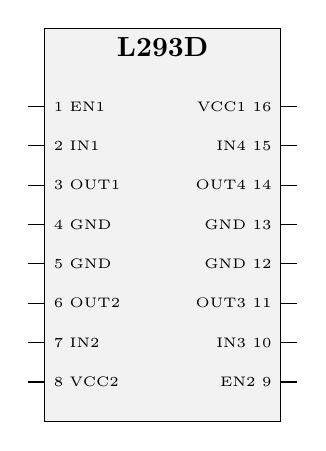
\begin{tikzpicture}[
    pin/.style={draw, rectangle, minimum width=2.5cm, minimum height=0.5cm, font=\tiny},
    ic/.style={draw, rectangle, minimum width=3cm, minimum height=5cm, fill=gray!10}
]
    \node [ic] (body) {};
    \node [anchor=north, font=\bfseries] at (body.north) {L293D};

    % Left pins
    \foreach \i/\label in {1/EN1, 2/IN1, 3/OUT1, 4/GND, 5/GND, 6/OUT2, 7/IN2, 8/VCC2} {
        \node [anchor=west, font=\tiny] at ([yshift=-0.5cm-\i*0.5cm]body.north west) {\i\ \label};
        \draw ([yshift=-0.5cm-\i*0.5cm]body.north west) -- +(-0.2,0);
    }
    
    % Right pins
    \foreach \i/\label in {16/VCC1, 15/IN4, 14/OUT4, 13/GND, 12/GND, 11/OUT3, 10/IN3, 9/EN2} {
        \pgfmathsetmacro{\ypos}{17-\i}
        \node [anchor=east, font=\tiny] at ([yshift=-0.5cm-\ypos*0.5cm]body.north east) {\label\ \i};
        \draw ([yshift=-0.5cm-\ypos*0.5cm]body.north east) -- +(0.2,0);
    }
\end{tikzpicture}
\end{center}

\begin{itemize}
    \item \keyword{Features}: Dual H-Bridge, 600mA per channel.
    \item \keyword{Operation}: Controls direction and speed (PWM).
    \item \keyword{Supply}: VCC1 logic (5V), VCC2 motor (up to 36V).
\end{itemize}
\end{solutionbox}

\begin{mnemonicbox}
\mnemonic{Dual-channel H-bridge Input-control Enable-PWM}
\end{mnemonicbox}

\orquestionmarks{5(c)}{7}{Explain Automatic Juice vending machine.}

\begin{solutionbox}
\textbf{Automatic Juice Vending Machine:}

\begin{answerdiagram}{Juice Vending Machine}
\begin{tikzpicture}[auto, node distance=2cm]
    \node [gtu block] (mcu) {ATmega32};
    \node [gtu block, left=of mcu] (keypad) {Keypad};
    \node [gtu block, above=of mcu] (lcd) {LCD Display};
    \node [gtu block, below=of mcu] (coin) {Coin\\Sensor};
    
    \node [gtu block, right=of mcu, yshift=1.5cm] (pump) {Pumps};
    \node [gtu block, right=of mcu, yshift=0cm] (valve) {Valves};
    \node [gtu block, right=of mcu, yshift=-1.5cm] (dispense) {Dispenser};
    
    \draw [gtu arrow] (keypad) -- (mcu);
    \draw [gtu arrow] (coin) -- (mcu);
    \draw [gtu arrow] (mcu) -- (lcd);
    \draw [gtu arrow] (mcu) -- (pump);
    \draw [gtu arrow] (mcu) -- (valve);
    \draw [gtu arrow] (pump) -- (dispense);
    \draw [gtu arrow] (valve) -- (dispense);
\end{tikzpicture}
\end{answerdiagram}

\textbf{Operation:}
\begin{enumerate}
    \item \keyword{Selection}: User selects juice via Keypad.
    \item \keyword{Payment}: Coin sensor validates payment.
    \item \keyword{Processing}: MCU activates pumps/valves for mixing.
    \item \keyword{Dispensing}: Juice is dispensed, message on LCD.
\end{enumerate}

\textbf{Features:} Multiple flavors, inventory monitoring, automated cleaning.
\end{solutionbox}

\begin{mnemonicbox}
\mnemonic{Juice-selection User-interface Mixing-control Payment-system Sensors-monitoring}
\end{mnemonicbox}

\end{document}
